\begin{abstract}

\textbf{Purpose.} This study develops a knowledge-enhanced Web
information system for Chinese-English railway vocational education,
enabling international learners to access terminology, regulations and
textbook knowledge with source traceability on limited local hardware.

\textbf{Design/methodology/approach.} The system combines an
approval-controlled PostgreSQL knowledge base, pgvector, BM25, BGE-M3,
reciprocal-rank fusion and local language models. A leakage-controlled
set of 400 bilingual knowledge pairs compares retrieval methods. Five
generators are tested under no-retrieval, BM25-RAG and
approved-hybrid-RAG conditions; QLoRA, directional translation and
deployment efficiency are evaluated separately on one 24 GB GPU.

\textbf{Findings.} Hybrid Recall@5 reached 0.715 in Chinese and 0.708 in
English. Qwen2.5 QLoRA raised held-out Char F1 from 0.189 to 0.398 in
Chinese and from 0.437 to 0.648 in English. RAG significantly improved
all generators, but adapted models often omitted evidence labels.
Translation gains were direction-dependent, and every deployment
condition remained below 20 GB peak memory.

\textbf{Originality.} The study integrates governed bilingual knowledge,
evidence-traceable RAG and resource-constrained deployment in a railway
Web information system. It reports language-disaggregated results and
implements expert approval as a query-time retrieval condition.

\textbf{Keywords:} knowledge-enhanced large language models; Web
information systems; retrieval-augmented generation; bilingual
education; railway vocational education; pgvector

\end{abstract}

\section{Introduction}\label{introduction}

Railway vocational education combines safety-critical regulations,
specialised terminology and procedural textbook knowledge. International
students must often move between Chinese source material and English
learning support. Generic large language models can produce fluent
answers, but their parametric knowledge does not expose a stable
boundary between verified railway knowledge and unsupported generation.
This is a Web information system problem as much as a model problem:
knowledge must be acquired, governed, retrieved, presented and traced to
its source.

The problem has practical importance beyond classroom convenience.
Railway technology, construction standards and operational expertise
increasingly circulate across linguistic and national boundaries, while
vocational institutions educate learners who may understand technical
concepts through English but must ultimately work with Chinese source
regulations. A useful service must therefore do more than translate
isolated terms. It must connect a bilingual question to the correct
version of a regulation or teaching passage, preserve provenance,
distinguish reviewed from unreviewed content and provide an answer
quickly enough for repeated learning and operational-training use.
Transportation studies have begun to explore specialised language models
for safety, rail design, track management, prognostics and driver advice
(Zheng et al., 2023; Lahnalampi, 2024; Wang and Li, 2024; Song et al.,
2025; Luo et al., 2025), while broader reviews identify reliability and
deployment as continuing challenges (Wandelt et al., 2024). Bilingual
educational access and resource-bounded governance nevertheless remain
under-examined.

Existing studies commonly evaluate either general-purpose language
models or retrieval-augmented generation in isolation. Four gaps
motivate this work. First, bilingual educational retrieval is rarely
evaluated separately by query language. Second, expert review is often
described as preprocessing rather than implemented as a queryable
governance state. Third, domain adaptation is frequently evaluated only
on the target task, leaving translation regressions and
citation-following failures hidden. Fourth, deployment studies often
omit the interaction between retrieval quality, answer traceability and
resource constraints on ordinary institutional hardware.

This study addresses the following research questions:

\begin{itemize}
\tightlist
\item
  \textbf{RQ1:} How accurately do BM25, pgvector dense retrieval and
  hybrid fusion retrieve held-out evidence for Chinese and English
  railway questions?
\item
  \textbf{RQ2:} How do retrieval strategy and expert-approved filtering
  affect answer quality, citation coverage and hallucination risk?
\item
  \textbf{RQ3:} What bilingual translation quality is achieved in each
  direction, and how does completion-only QLoRA affect domain QA without
  contaminating the held-out test set?
\item
  \textbf{RQ4:} Can the resulting system operate within the latency and
  memory constraints of a single 24 GB GPU workstation?
\end{itemize}

The study makes four contributions. First, it operationalises a
bilingual railway knowledge base in which review state, source metadata,
language variants and revision history remain queryable rather than
being flattened into an anonymous vector collection. Second, it develops
a PostgreSQL/pgvector Web information system that combines lexical and
multilingual dense retrieval with evidence-labelled local generation.
Third, it introduces a pair-grouped, leakage-controlled protocol that
separates Chinese and English retrieval, QA and translation outcomes.
Fourth, it evaluates adaptation, retrieval and deployment jointly,
exposing both quality gains and failures in citation following,
directional translation and resource use.

\section{Related work}\label{related-work}

\subsection{Knowledge-enhanced Web information
systems}\label{knowledge-enhanced-web-information-systems}

Web information systems increasingly combine structured data management,
semantic access and generative interfaces. Retrieval-augmented
generation (RAG) provides a practical separation between parametric
generation and an externally maintained evidence collection (Lewis et
al., 2020). This separation is relevant to institutional knowledge
systems because source records can be revised without retraining the
generator. It does not, however, guarantee faithful generation:
retrieval can miss the relevant record, and a generator can still
misrepresent correctly retrieved evidence. The present study therefore
evaluates retrieval, answer overlap, evidence hit and citation behaviour
as distinct outcomes.

The retrieval layer combines complementary lexical and semantic signals.
BM25 remains an efficient lexical baseline for exact domain terms
(Robertson and Zaragoza, 2009), while reciprocal-rank fusion can combine
rankings without requiring directly comparable score scales (Cormack et
al., 2009). PostgreSQL and pgvector place vector search beside governed
relational metadata, allowing approval state and held-out split
boundaries to be applied in the query rather than after generation. This
makes knowledge governance an executable part of the information-system
design.

This distinction separates the proposed system from a document-only RAG
demonstration. A Web information system must maintain record identity
and lifecycle state across ingestion, review, retrieval and
presentation. In this study the vector representation is derived data
attached to a governed record, not the primary source of truth.
Deleting, revising or withholding a record can therefore change
retrieval eligibility without rebuilding the entire application or
relying on prompt instructions to enforce governance.

\subsection{Retrieval-augmented generation in
education}\label{retrieval-augmented-generation-in-education}

Generative AI can support explanation, feedback and access to learning
resources, but education research has also identified risks involving
factual reliability, learner over-reliance and opaque provenance
(Kasneci et al., 2023; UNESCO, 2023). Educational RAG addresses part of
this problem by grounding responses in course or institutional material.
Many demonstrations nevertheless report a pooled answer score without
isolating retrieval failure, language effects or deployment cost. Such
aggregation is particularly problematic for international vocational
education, where an English query may need evidence originating in
Chinese regulations or textbooks. This study consequently reports
Chinese and English retrieval and generation separately and preserves
document-level provenance in every retrieved result.

Railway applications illustrate why this separation matters. RSChat
addresses railway safety question answering (Li et al., 2024), while
domain-specialised systems have been proposed for train-driver advice
and emergency-response generation (Luo et al., 2025; Huang et al.,
2026). These studies establish the value of domain knowledge, yet their
operational targets differ from multilingual learning: an international
learner may formulate a concept in English, retrieve a Chinese
regulation and require an answer that preserves both the translated
explanation and the original evidence. The present work therefore treats
cross-language access, provenance and constrained institutional
deployment as co-equal requirements.

\subsection{Bilingual domain adaptation and
evaluation}\label{bilingual-domain-adaptation-and-evaluation}

Bilingual domain systems require both cross-lingual retrieval and
controlled generation. BGE-M3 supports multilingual dense retrieval and
was selected to provide a shared embedding space for the Chinese and
English knowledge fields (Chen et al., 2024). Dense similarity is not
assumed to dominate lexical matching; the two methods are compared
independently before fusion.

Parameter-efficient adaptation provides a second mechanism for domain
specialisation. QLoRA trains low-rank adapters through a frozen 4-bit
quantised base model, reducing memory requirements while retaining task
adaptation capacity (Dettmers et al., 2023). In this study,
completion-only masking prevents the prompt from contributing to the
training loss, and bilingual variants sharing a knowledge-pair
identifier remain in the same split. Translation is evaluated
directionally because Chinese-to-English and English-to-Chinese scores
are not interchangeable. Terminology and complete-sentence translation
are also kept separate.

PEFT methods reduce trainable parameters but do not guarantee a better
deployed system (Ding et al., 2023; Wang et al., 2025). Limited-resource
training remains sensitive to quantisation, sequence length, optimiser
state and model-specific target modules (Lv et al., 2024). Moreover,
task adaptation can improve answer overlap while degrading factuality,
instruction following or unrelated capabilities (Tian et al., 2024;
Barnett et al., 2024). This motivates the present before-and-after
design, which reports not only domain QA but also general-capability
checks, citation behaviour and memory use.

Domain translation creates a further risk of pooled evaluation. Prior
work shows that fine-tuning effects depend on training direction, domain
composition and data volume (Hu et al., 2024; Vieira et al., 2024; Zheng
et al., 2024). Consequently, this study does not interpret a single
bilingual mean as evidence of robust translation. It reports terminology
and sentence tasks independently in both directions and retains empty or
wrong-language outputs as failures rather than silently discarding them.

\subsection{Research gap and analytical
framework}\label{research-gap-and-analytical-framework}

The literature suggests that domain retrieval, adaptation and local
deployment are individually feasible, but it does not establish that
their benefits compose monotonically. The analytical framework therefore
treats the system as four testable layers: governed knowledge,
retrieval, generation/adaptation and deployment. A failure at one layer
cannot be compensated for statistically by a high score at another.
Retrieval recall is measured before answer generation; citation-format
compliance is separated from answer overlap; translation is separated
from QA; and quality is reported alongside latency and memory. This
layered design provides the basis for answering RQ1-RQ4 without
attributing every observed change to the language model alone.

\section{System design and research
method}\label{system-design-and-research-method}

\subsection{Application context and
requirements}\label{application-context-and-requirements}

The target users are railway vocational teachers, Chinese-speaking
learners and international students requiring English support. The
system must return concise answers, expose numbered evidence, preserve
document metadata and run locally where cloud use is restricted.

Requirements were organised around three user-facing workflows. Learners
submit a Chinese or English question, inspect an answer and open its
evidence records. Teachers search or edit bilingual knowledge, inspect
source metadata and route records through review. Administrators
maintain model, embedding and database services and monitor whether a
response can be generated within local resource limits. These workflows
produced five design requirements: bilingual access, source
traceability, review-state enforcement, held-out-data isolation and
deployability on one workstation. The architecture in Figure 1 maps each
requirement to a persistent or testable component rather than treating
them as prompt-level behaviour.

\subsection{Expert-governed knowledge
base}\label{expert-governed-knowledge-base}

Knowledge records include Chinese and English questions and answers,
evidence, original text, source document, chapter, page, task type,
quality flags, review status and revision history. PostgreSQL stores
governed records; pgvector stores 1,024-dimensional BGE-M3 embeddings.
The production index excludes the held-out test split.

The knowledge sources comprise railway terminology, operating and safety
regulations, and vocational textbook or concept material. Ingestion
preserves source-document, chapter and page fields whenever available.
Chinese and English questions and answers are stored in separate fields
on the same logical record so that a language variant does not lose its
source identity. Embeddings are linked by record identifier and model
revision; they can be rebuilt without changing the reviewed text. A
record marked \texttt{rejected}, \texttt{needs\_revision} or as part of
the frozen RAG test is excluded before ranking. This database-level
decision prevents held-out evidence from leaking through either BM25 or
vector retrieval.

Knowledge review is conducted by experts drawn from front-line railway
education and international education. Their role is to assess domain
correctness, educational suitability, bilingual expression and
consistency with the cited source before a record becomes eligible for
approved-only retrieval. Expert names, exact panel size, experience
distribution, assignment procedure and agreement statistics will be
completed together after the expert-information collection is closed.
\textbf{{[}Expert metadata to complete before submission: panel size;
railway specialisms; years of teaching; international-education roles;
number of reviewers per record; disagreement-resolution rule; agreement
statistic where available.{]}} No uncollected value is inferred in the
present draft. Accordingly, \texttt{approved} is analysed as an
operational governance state, not as proof of unanimous expert
consensus.

\begin{figure}
\centering
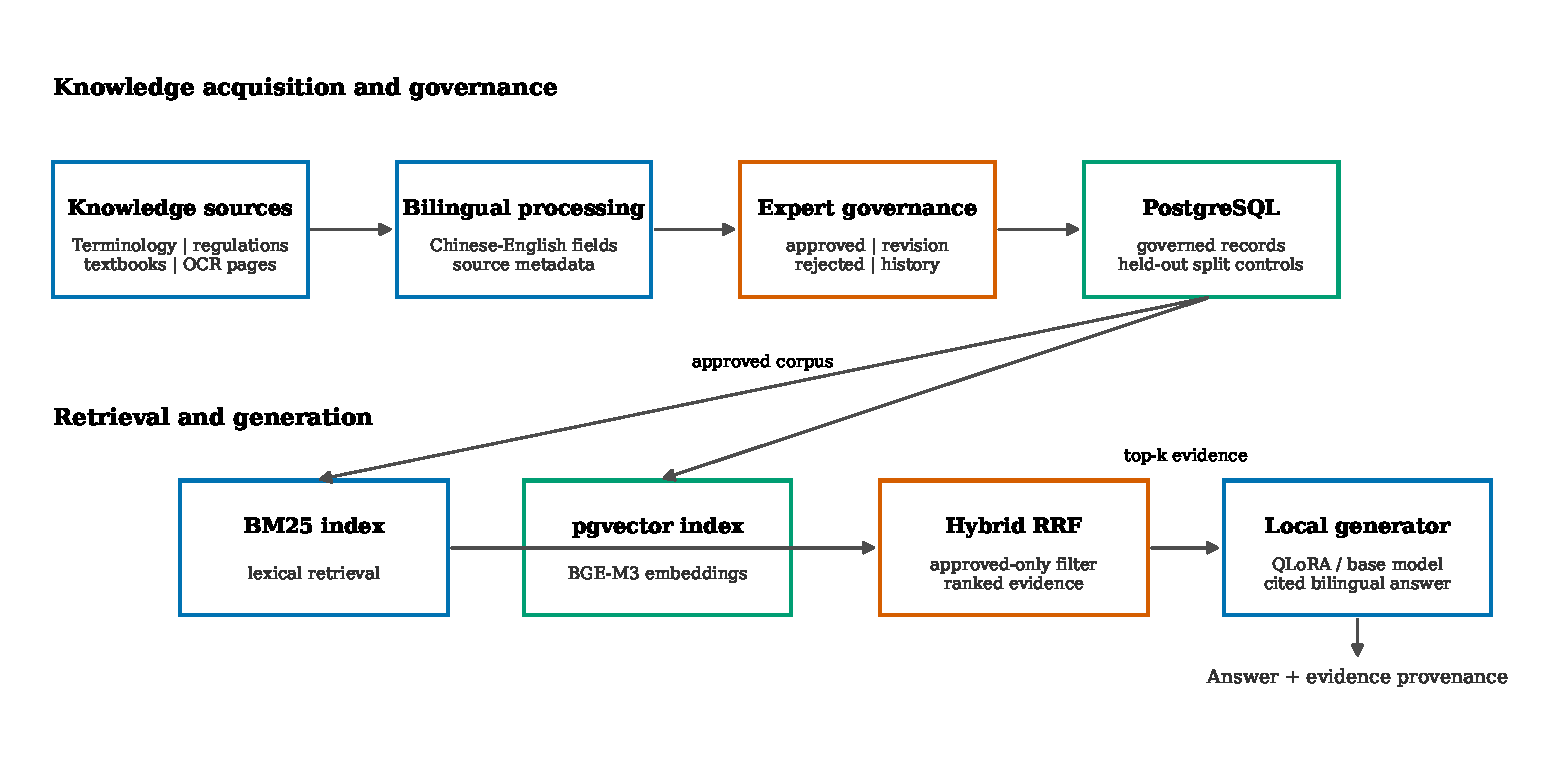
\includegraphics[width=0.96\linewidth,height=\textheight,keepaspectratio]{../paper/ijwis/figures/system_architecture.pdf}
\caption{System architecture and knowledge-governance workflow.}
\end{figure}

\subsection{Retrieval and answer
generation}\label{retrieval-and-answer-generation}

BM25 indexes Chinese and English question-answer fields and evidence.
Dense search embeds a query with BGE-M3 and ranks chunks by vector
similarity. Hybrid retrieval fuses keyword and dense rankings using
reciprocal-rank fusion. The \texttt{approved\_only} condition applies
expert status as a database-level filter. Retrieved evidence is numbered
and supplied to the local generator with an instruction to answer in the
query language and cite evidence labels.

For a candidate document \emph{d}, the fusion score is:

\begin{equation}
\operatorname{RRF}(d)=\sum_{r \in \{\mathrm{BM25},\mathrm{vector}\}}\frac{1}{k_0+\operatorname{rank}_r(d)}.
\end{equation}

The candidate pool is fixed at 50 per retriever and the conventional
rank constant is \texttt{k0\ =\ 60}; final top-\emph{k} is varied only
after fusion. This separation ensures that a top-\emph{k} ablation
changes the amount of evidence delivered to the generator without
changing the upstream search pool. Dense ranking uses BGE-M3 query
embeddings and pgvector distance, while lexical ranking retains exact
matches that are valuable for abbreviations, equipment names and
regulation numbers. Every returned evidence object contains record
identifier, source document, task type and retrieval score.

The FastAPI service exposes search and conversational endpoints to the
Web client. At answer time, the selected evidence is serialised with
labels such as \texttt{{[}Evidence1{]}} or \texttt{{[}证据1{]}}. The
system instruction requires the generator to answer in the query
language, remain within the supplied evidence and attach labels to
supported statements. If no admissible record is retrieved, the service
returns an explicit no-evidence message rather than invoking
unconstrained generation. Figure 1 shows the resulting acquisition,
governance, retrieval and generation path.

\subsection{Bilingual QLoRA
adaptation}\label{bilingual-qlora-adaptation}

The adaptation dataset is generated only from approved records and split
by knowledge-pair identifier, task type and source document. Chinese and
English variants of the same knowledge item are assigned to the same
partition. The current frozen 80/10/10 corpus contains 12,178 training,
1,524 validation and 1,526 test examples, balanced equally by language,
with zero pair overlap among all partitions. The 120 regulation items
reserved for RAG evaluation are forced into the test partition and never
used for training. Loss is computed only on answer tokens; all prompt
labels are masked with \texttt{-100}.

Qwen2.5-7B-Instruct and GLM-4-9B-Chat-HF form the adaptation matrix.
Both were loaded with NF4 quantisation and PEFT adapters on the target
GPU. Qwen exposes separate \texttt{gate\_proj} and \texttt{up\_proj}
modules, whereas GLM uses a fused \texttt{gate\_up\_proj};
model-specific target lists are therefore required. The formal rank-64
configuration trained 161,480,704 Qwen parameters and 190,382,080 GLM
parameters, representing 3.58 and 3.45 per cent of the parameters
visible to the quantised training process, respectively.

Both runs use LoRA rank 64, alpha 16, dropout 0.05, learning rate
\texttt{2e-4}, maximum sequence length 1,024 and one epoch. The
per-device batch size is one with 16 gradient-accumulation steps and a
0.03 warm-up ratio. Random seed 42 is fixed in the experiment
configuration. Generation uses greedy decoding
(\texttt{temperature\ =\ 0}, \texttt{top\_p\ =\ 1}) with a
task-dependent output limit. Completion-only supervision masks every
prompt token with \texttt{-100}; therefore, training optimises the
answer sequence rather than teaching the model to reproduce
instructions. This choice is tested rather than assumed to improve every
downstream behaviour.

\subsection{Evaluation design}\label{evaluation-design}

Retrieval conditions are BM25, vector, hybrid and approved hybrid.
Metrics are Recall@1/3/5, MRR and mean latency. The regulation pilot
includes six answer conditions; the formal generator matrix fixes no
retrieval, BM25-RAG and approved hybrid-RAG so that five generators
receive identical cached contexts. Automatic metrics include answer F1,
reference containment, citation-format coverage, a citation-format-based
hallucination proxy and end-to-end latency. Citation measures are
treated as instruction-following proxies, not evidence entailment.
Translation is reported independently for Chinese-to-English and
English-to-Chinese terminology and sentences using SacreBLEU, chrF++ and
COMET (\texttt{Unbabel/wmt22-comet-da}). This multi-dimensional protocol
follows the broader principle that LLM evaluation should separate task
capability, robustness and deployment behaviour rather than rely on one
aggregate score (Chang et al., 2024).

Recall@\emph{k} is one when the held-out source record occurs in the
first \emph{k} positions and zero otherwise; MRR averages the reciprocal
rank of the first relevant record. Character-level F1 is used for
Chinese and token-normalised overlap for English. Reference containment
records whether the normalised reference appears in the generated
answer. Citation coverage records only whether the requested
evidence-label syntax appears. The hallucination proxy is zero when a
recognised no-evidence response or citation label is present and one
otherwise; it is deliberately named a proxy because it does not test
claim-evidence entailment. This limitation is retained in every
interpretation.

All core comparisons use paired samples. Mean metrics are accompanied by
2,000-resample bootstrap 95 per cent confidence intervals.
Original-versus-QLoRA comparisons use two-sided paired Wilcoxon tests,
paired standardised effect sizes and Holm correction across the
pre-specified comparison family. Exploratory error categories are
reported separately and are not treated as confirmatory hypothesis
tests. Efficiency measurements use 30 Chinese short questions, 30
English short questions and 30 regulation-oriented long-context
questions, with one warm-up and three measured repetitions per model
condition.

\subsection{Implementation and
reproducibility}\label{implementation-and-reproducibility}

The application uses a Vite-based Web client, a FastAPI backend and
PostgreSQL 16.14 with pgvector 0.8.4. Experiments ran on Linux with an
NVIDIA GeForce RTX 3090 (24,576 MiB), 32 GB host memory, Python 3.11.15,
PyTorch 2.11.0, Transformers 5.12.1, PEFT 0.18.1 and bitsandbytes
0.49.2. Qwen2.5-7B-Instruct, GLM-4-9B-Chat-HF and BGE-M3 are pinned by
model revision in the frozen manifest. COMET uses the pinned
\texttt{Unbabel/wmt22-comet-da} checkpoint. Input datasets,
configurations, generated tables and final analysis assets are recorded
with SHA-256 hashes.

\textbf{Table 1. Formal implementation and experimental environment.}

{\def\LTcaptype{none} % do not increment counter
\begin{longtable}[]{@{}
  >{\raggedright\arraybackslash}p{(\linewidth - 2\tabcolsep) * \real{0.5000}}
  >{\raggedright\arraybackslash}p{(\linewidth - 2\tabcolsep) * \real{0.5000}}@{}}
\toprule\noalign{}
\begin{minipage}[b]{\linewidth}\raggedright
Component
\end{minipage} & \begin{minipage}[b]{\linewidth}\raggedright
Formal setting
\end{minipage} \\
\midrule\noalign{}
\endhead
\bottomrule\noalign{}
\endlastfoot
Database & PostgreSQL 16.14; pgvector 0.8.4 \\
Embedding & BAAI/bge-m3; 1,024 dimensions \\
Adapted generators & Qwen2.5-7B-Instruct; GLM-4-9B-Chat-HF \\
Reference generator & Qwen3-14B through Ollama 0.19.0 \\
Training & NF4 QLoRA; rank 64; one epoch; seed 42 \\
Hardware & RTX 3090 24 GB; 32 GB RAM; single workstation \\
Statistical analysis & 2,000 bootstrap resamples; paired Wilcoxon; Holm
correction \\
\end{longtable}
}

The code separates test-set construction, embedding, retrieval
evaluation, generator evaluation, adaptation and report export. This
prevents an analysis script from silently changing the production index
or training split. Cached retrieval contexts are reused across
generators in the formal RAG matrix, so model comparisons receive
identical evidence. The manifest records the Git state and every input
hash at freeze time, supporting result reconstruction even when
copyrighted source passages cannot be redistributed.

\section{Results}\label{results}

\subsection{Knowledge-base
composition}\label{knowledge-base-composition}

The database contains 37,661 approved records and 37,109 complete
bilingual records. After freezing the formal RAG test, 37,261 approved
non-test knowledge chunks have BGE-M3 embeddings. The QLoRA test
partition contains 763 knowledge pairs across four source documents.
From this partition, the formal cross-source RAG set contains 400
knowledge pairs and 800 language-specific queries: 150 regulation, 127
terminology and 123 textbook/concept pairs across 17 task types. The
original 120 regulation pairs remain a separately reported specialised
subset.

\subsection{Regulation-only pilot
retrieval}\label{regulation-only-pilot-retrieval}

\textbf{Table 2. Regulation-only pilot retrieval results.}

{\def\LTcaptype{none} % do not increment counter
\begin{longtable}[]{@{}
  >{\raggedright\arraybackslash}p{(\linewidth - 12\tabcolsep) * \real{0.1111}}
  >{\raggedleft\arraybackslash}p{(\linewidth - 12\tabcolsep) * \real{0.1481}}
  >{\raggedleft\arraybackslash}p{(\linewidth - 12\tabcolsep) * \real{0.1481}}
  >{\raggedleft\arraybackslash}p{(\linewidth - 12\tabcolsep) * \real{0.1481}}
  >{\raggedleft\arraybackslash}p{(\linewidth - 12\tabcolsep) * \real{0.1481}}
  >{\raggedleft\arraybackslash}p{(\linewidth - 12\tabcolsep) * \real{0.1481}}
  >{\raggedleft\arraybackslash}p{(\linewidth - 12\tabcolsep) * \real{0.1481}}@{}}
\toprule\noalign{}
\begin{minipage}[b]{\linewidth}\raggedright
Retrieval
\end{minipage} & \begin{minipage}[b]{\linewidth}\raggedleft
Language
\end{minipage} & \begin{minipage}[b]{\linewidth}\raggedleft
R@1
\end{minipage} & \begin{minipage}[b]{\linewidth}\raggedleft
R@3
\end{minipage} & \begin{minipage}[b]{\linewidth}\raggedleft
R@5
\end{minipage} & \begin{minipage}[b]{\linewidth}\raggedleft
MRR
\end{minipage} & \begin{minipage}[b]{\linewidth}\raggedleft
Mean latency (ms)
\end{minipage} \\
\midrule\noalign{}
\endhead
\bottomrule\noalign{}
\endlastfoot
BM25 & Chinese & 0.625 & 0.708 & 0.742 & 0.672 & 48.7 \\
Vector & Chinese & 0.575 & 0.717 & 0.742 & 0.648 & 125.4 \\
Hybrid approved & Chinese & \textbf{0.667} & \textbf{0.717} &
\textbf{0.758} & \textbf{0.701} & 185.0 \\
BM25 & English & 0.517 & 0.642 & 0.667 & 0.580 & 70.0 \\
Vector & English & 0.483 & 0.567 & 0.575 & 0.523 & 361.7 \\
Hybrid approved & English & \textbf{0.525} & \textbf{0.667} &
\textbf{0.708} & \textbf{0.595} & 185.7 \\
\end{longtable}
}

In this regulation-only pilot, hybrid retrieval gives the strongest
Recall@5 in both languages. English queries remain consistently harder,
which supports reporting language-disaggregated results rather than a
pooled bilingual score. These values will not be treated as the final
cross-source system results.

\subsection{Formal cross-source bilingual
retrieval}\label{formal-cross-source-bilingual-retrieval}

\textbf{Table 3. Formal cross-source retrieval on 400 knowledge pairs.}

{\def\LTcaptype{none} % do not increment counter
\begin{longtable}[]{@{}
  >{\raggedright\arraybackslash}p{(\linewidth - 12\tabcolsep) * \real{0.1111}}
  >{\raggedleft\arraybackslash}p{(\linewidth - 12\tabcolsep) * \real{0.1481}}
  >{\raggedleft\arraybackslash}p{(\linewidth - 12\tabcolsep) * \real{0.1481}}
  >{\raggedleft\arraybackslash}p{(\linewidth - 12\tabcolsep) * \real{0.1481}}
  >{\raggedleft\arraybackslash}p{(\linewidth - 12\tabcolsep) * \real{0.1481}}
  >{\raggedleft\arraybackslash}p{(\linewidth - 12\tabcolsep) * \real{0.1481}}
  >{\raggedleft\arraybackslash}p{(\linewidth - 12\tabcolsep) * \real{0.1481}}@{}}
\toprule\noalign{}
\begin{minipage}[b]{\linewidth}\raggedright
Retrieval
\end{minipage} & \begin{minipage}[b]{\linewidth}\raggedleft
Language
\end{minipage} & \begin{minipage}[b]{\linewidth}\raggedleft
R@1
\end{minipage} & \begin{minipage}[b]{\linewidth}\raggedleft
R@3
\end{minipage} & \begin{minipage}[b]{\linewidth}\raggedleft
R@5
\end{minipage} & \begin{minipage}[b]{\linewidth}\raggedleft
MRR
\end{minipage} & \begin{minipage}[b]{\linewidth}\raggedleft
Mean latency (ms)
\end{minipage} \\
\midrule\noalign{}
\endhead
\bottomrule\noalign{}
\endlastfoot
BM25 & Chinese & 0.520 & 0.595 & 0.620 & 0.560 & \textbf{69.5} \\
Vector & Chinese & 0.518 & 0.653 & 0.690 & 0.588 & 134.4 \\
Hybrid approved & Chinese & \textbf{0.570} & \textbf{0.675} &
\textbf{0.715} & \textbf{0.628} & 217.6 \\
BM25 & English & \textbf{0.570} & \textbf{0.670} & 0.685 & 0.620 &
\textbf{59.0} \\
Vector & English & 0.463 & 0.553 & 0.580 & 0.509 & 134.4 \\
Hybrid approved & English & \textbf{0.570} & 0.668 & \textbf{0.708} &
\textbf{0.620} & 209.2 \\
\end{longtable}
}

The larger cross-source evaluation changes the interpretation of the
pilot. BM25 is particularly competitive for English terminology queries,
while dense retrieval contributes more strongly to Chinese evidence
recall. With the RRF candidate pool fixed at 50 for every final cutoff,
hybrid fusion obtains the highest Recall@5 in both languages, although
its latency is approximately three times that of BM25. Increasing the
final cutoff from three to eight raises approved-hybrid recall from
0.675 to 0.743 in Chinese and from 0.668 to 0.723 in English, while mean
retrieval latency remains nearly constant because the candidate pool is
controlled (Figure 2). Approved-only and unfiltered hybrid results are
identical because all admissible indexed records in this frozen
experiment satisfy the approval condition.

\begin{figure}
\centering
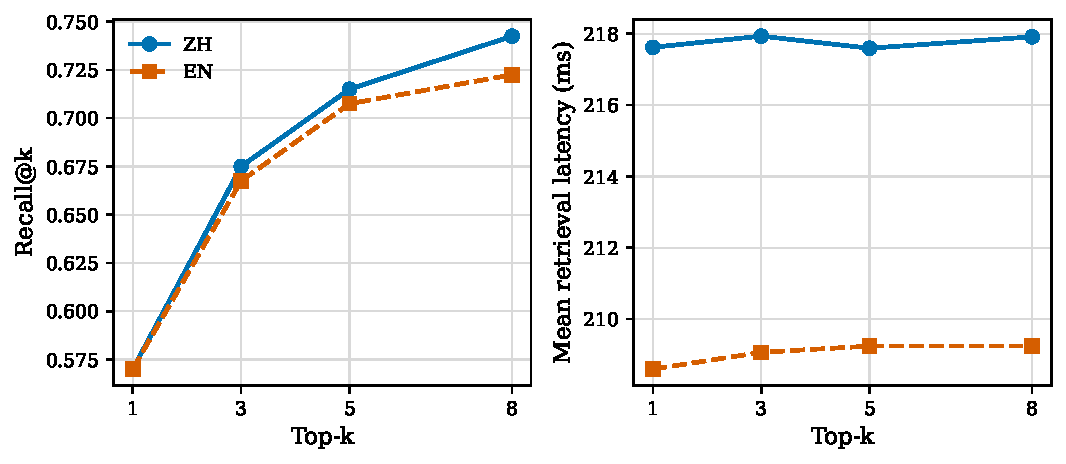
\includegraphics[width=0.96\linewidth,height=\textheight,keepaspectratio]{../paper/ijwis/figures/top_k_quality_latency.pdf}
\caption{Approved-hybrid retrieval quality and latency across top-k
settings.}
\end{figure}

\subsection{Regulation-only pilot answer
generation}\label{regulation-only-pilot-answer-generation}

\textbf{Table 4. Regulation-only answer-generation results.}

{\def\LTcaptype{none} % do not increment counter
\begin{longtable}[]{@{}
  >{\raggedright\arraybackslash}p{(\linewidth - 10\tabcolsep) * \real{0.1304}}
  >{\raggedleft\arraybackslash}p{(\linewidth - 10\tabcolsep) * \real{0.1739}}
  >{\raggedleft\arraybackslash}p{(\linewidth - 10\tabcolsep) * \real{0.1739}}
  >{\raggedleft\arraybackslash}p{(\linewidth - 10\tabcolsep) * \real{0.1739}}
  >{\raggedleft\arraybackslash}p{(\linewidth - 10\tabcolsep) * \real{0.1739}}
  >{\raggedleft\arraybackslash}p{(\linewidth - 10\tabcolsep) * \real{0.1739}}@{}}
\toprule\noalign{}
\begin{minipage}[b]{\linewidth}\raggedright
Condition
\end{minipage} & \begin{minipage}[b]{\linewidth}\raggedleft
Language
\end{minipage} & \begin{minipage}[b]{\linewidth}\raggedleft
Answer F1
\end{minipage} & \begin{minipage}[b]{\linewidth}\raggedleft
Citation coverage
\end{minipage} & \begin{minipage}[b]{\linewidth}\raggedleft
Hallucination proxy
\end{minipage} & \begin{minipage}[b]{\linewidth}\raggedleft
End-to-end (ms)
\end{minipage} \\
\midrule\noalign{}
\endhead
\bottomrule\noalign{}
\endlastfoot
No retrieval & Chinese & 0.243 & 0.000 & 1.000 & 3,243.1 \\
BM25-RAG & Chinese & \textbf{0.621} & 0.967 & 0.033 &
\textbf{1,141.8} \\
Vector-RAG & Chinese & 0.623 & 0.967 & 0.033 & 1,149.4 \\
Hybrid-RAG approved & Chinese & 0.604 & \textbf{0.975} & \textbf{0.025}
& 1,413.8 \\
No retrieval & English & 0.243 & 0.000 & 1.000 & 3,495.5 \\
BM25-RAG & English & \textbf{0.498} & \textbf{0.992} & \textbf{0.008} &
\textbf{1,322.5} \\
Vector-RAG & English & 0.492 & 0.950 & 0.050 & 1,425.4 \\
Hybrid-RAG approved & English & 0.489 & \textbf{0.992} & \textbf{0.008}
& 1,586.2 \\
\end{longtable}
}

RAG more than doubled F1 relative to no retrieval in both languages
while reducing mean response time because evidence-constrained answers
were shorter. Hybrid retrieval obtained the strongest evidence recall,
but this did not translate into the highest answer F1; BM25-RAG was the
strongest English generation condition and vector-RAG was marginally
strongest in Chinese. This distinction supports evaluating retrieval and
generation separately. Retrieval-only returned source-language evidence
and is therefore excluded from the generative comparison, particularly
for English questions.

\subsection{QLoRA adaptation and held-out
QA}\label{qlora-adaptation-and-held-out-qa}

Both one-epoch training runs converged without interruption. Qwen
trained for 3,546 s (59.1 min), with final training and validation
losses of 0.950 and 0.720 and peak reserved memory of 13.0 GB. GLM
trained for 4,571 s (76.2 min), with losses of 1.146 and 0.794 and peak
reserved memory of 15.0 GB. The respective validation perplexities were
2.05 and 2.21.

Figure 3 presents the training and validation trajectories. Because each
model was trained for one epoch, the curves establish completion and
optimisation behaviour rather than convergence across repeated
schedules. The absence of an extended hyperparameter search is
consistent with the resource-constrained design but limits claims about
globally optimal adapter settings.

On the 1,526-example held-out bilingual QA set, Qwen QLoRA increased
Char F1 from 0.189 (95 per cent CI 0.175-0.204) to 0.398 (0.376-0.422)
in Chinese and from 0.437 (0.419-0.455) to 0.648 (0.632-0.664) in
English. GLM increased from 0.192 to 0.410 in Chinese and from 0.498 to
0.552 in English. All four paired gains remained significant after Holm
correction (\texttt{p} \textless{} 0.000001); paired effect sizes were
0.569 and 0.634 for Qwen Chinese and English, and 0.614 and 0.146 for
GLM. Qwen therefore provides the strongest balanced adapted QA result,
while the small GLM English effect cautions against pooling languages.

A limited general-capability check (maximum 200 examples per subtask)
found that Qwen C-Eval/MMLU accuracy changed from 0.788/0.739 to
0.775/0.728, whereas GLM changed from 0.675/0.673 to 0.683/0.679. These
small changes do not indicate broad catastrophic forgetting, but the
limited protocol is a regression check rather than a comprehensive
general benchmark.

\begin{figure}
\centering
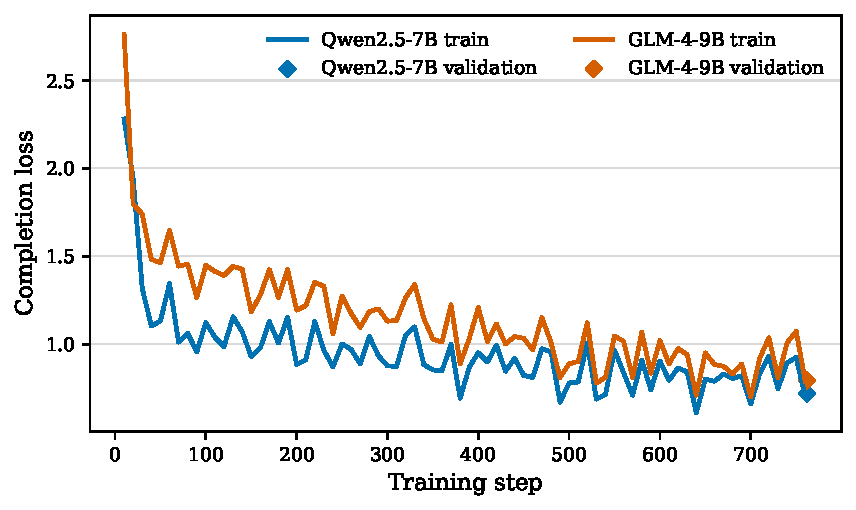
\includegraphics[width=0.96\linewidth,height=\textheight,keepaspectratio]{../paper/ijwis/figures/training_validation_loss.pdf}
\caption{Completion-only QLoRA training and validation loss.}
\end{figure}

\subsection{Multi-generator RAG and interaction
effects}\label{multi-generator-rag-and-interaction-effects}

Approved hybrid RAG significantly improved Answer F1 over no retrieval
for every generator and language after Holm correction. For original
Qwen, F1 rose from 0.262 to 0.402 in Chinese and from 0.306 to 0.440 in
English (paired effect sizes 0.796 and 0.798). Qwen QLoRA achieved the
highest absolute RAG F1, 0.660 in Chinese and 0.651 in English,
exceeding the Qwen3-14B reference values of 0.442 and 0.454. However,
its incremental hybrid-RAG gains over no retrieval were only 0.030 and
0.078, compared with 0.141 and 0.133 for original Qwen. Adaptation and
retrieval are therefore complementary in answer overlap, but with
diminishing returns.

The traceability result points in the opposite direction. Approved
hybrid citation-format coverage was 0.595/0.643 for original Qwen and
0.788/0.905 for Qwen3 in Chinese/English, but 0.000/0.003 for Qwen
QLoRA. GLM showed the same, less extreme pattern. QLoRA specialised
answer content while weakening compliance with a citation instruction
absent from its training targets. The citation-based hallucination proxy
consequently approaches one for adapted models and must not be read as a
factual hallucination rate. For an operational system, Qwen2.5 QLoRA is
the primary answer-quality model, while original Qwen or Qwen3 remains
the safer traceability control until citation-aware adaptation is added.

\subsection{Directional translation}\label{directional-translation}

Translation effects were direction- and task-dependent. Qwen COMET moved
from 0.501 to 0.509 for Chinese-to-English terminology and from 0.610 to
0.614 for English-to-Chinese sentences, but fell from 0.656 to 0.599 for
Chinese-to-English sentences and from 0.596 to 0.485 for
English-to-Chinese terminology. Its lexical metrics show the same lack
of uniform benefit: Chinese-to-English terminology chrF++ increased from
10.41 to 16.69, whereas sentence chrF++ fell from 47.43 to 31.28.

Figure 4 visualises the before-and-after COMET changes by direction and
task. The opposing slopes demonstrate why the result cannot be
summarised as a single improvement or regression.

GLM QLoRA is a clear failure case. Its sentence COMET dropped from 0.667
to 0.348 for Chinese-to-English and from 0.742 to 0.343 for
English-to-Chinese; corpus BLEU was zero in both directions. Automated
inspection found 2,168 empty outputs among 2,634 translation examples
(82.3 per cent). This result rules out a claim that QA-oriented
completion-only adaptation generally improves translation and shows why
terminology and sentence translation must remain separate from QA
evaluation.

\begin{figure}
\centering
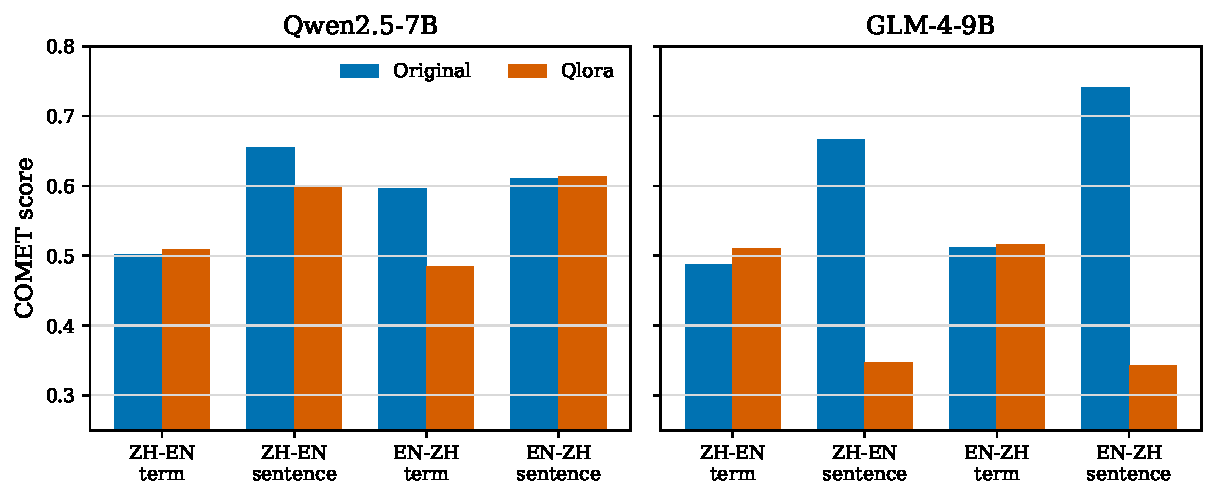
\includegraphics[width=0.96\linewidth,height=\textheight,keepaspectratio]{../paper/ijwis/figures/translation_before_after.pdf}
\caption{Direction- and task-separated COMET before and after QLoRA.}
\end{figure}

\subsection{Resource use and automated error
analysis}\label{resource-use-and-automated-error-analysis}

All five deployment conditions completed 270 measurements without
failure or OOM. Original Qwen and GLM used 5.49 and 6.76 GB peak
reserved memory and generated at 31.9 and 22.7 tokens/s. Their QLoRA
variants used 16.11 and 19.49 GB and generated at 17.5 and 11.9
tokens/s. Qwen3-14B through Ollama used 14.26 GB and 78.5 tokens/s,
although cross-backend timing should be interpreted cautiously. The Qwen
and GLM adapters occupy approximately 627 and 746 MB. The low 2.63 s GLM
QLoRA mean latency reflects abnormally short or empty outputs and is not
an efficiency advantage. All configurations fit the target 24 GB
workstation, but original Qwen provides the lowest resource cost and
Qwen QLoRA the strongest QA quality within the limit.

The quality-latency-memory relationship is shown in Figure 5. The plot
is interpreted as a deployment frontier rather than a universal model
ranking because Ollama and Hugging Face use different inference
backends.

Automated failure flags explain several aggregate differences. At top
three, approved hybrid retrieval missed the held-out item for 32.5 per
cent of Chinese and 33.3 per cent of English queries. Even with a hit,
original Qwen produced low-overlap answers in 18.0 per cent of Chinese
versus 4.3 per cent of English cases. Qwen QLoRA reduced these rates to
4.0 and 1.5 per cent, but omitted citation labels in 100.0 and 99.8 per
cent. Figure 6 compares these automatically flagged categories. The
translation analysis additionally exposed empty answers, wrong-language
outputs and terminology substitutions. Similar-version retrieval and
citation entailment require expert semantic judgement and were not
inferred from string-based flags.

\begin{figure}
\centering
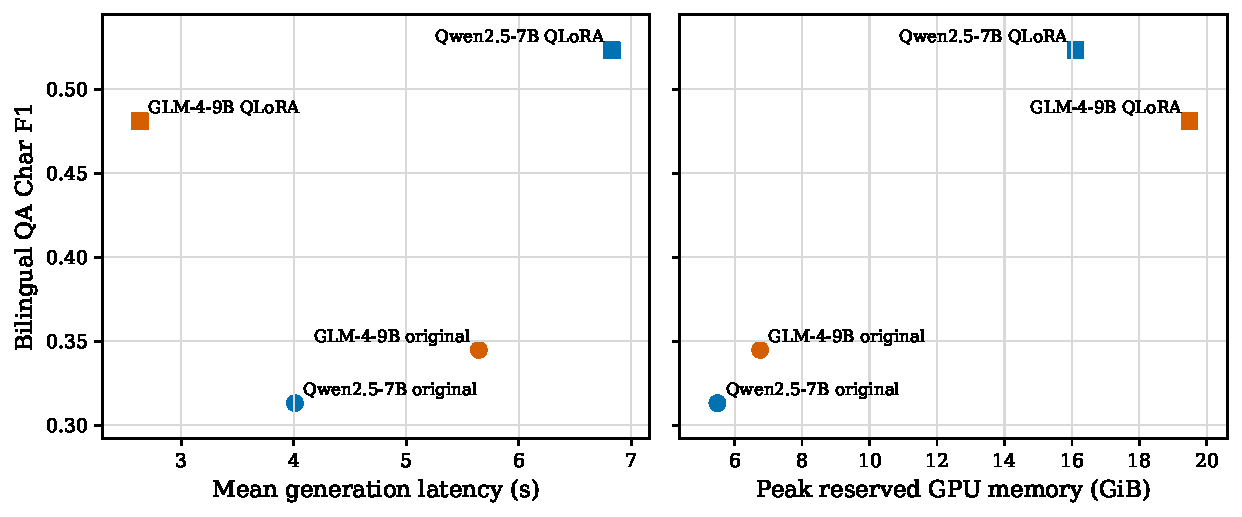
\includegraphics[width=0.96\linewidth,height=\textheight,keepaspectratio]{../paper/ijwis/figures/quality_latency_pareto.pdf}
\caption{Bilingual QA quality against generation latency and peak GPU
memory.}
\end{figure}

\begin{figure}
\centering
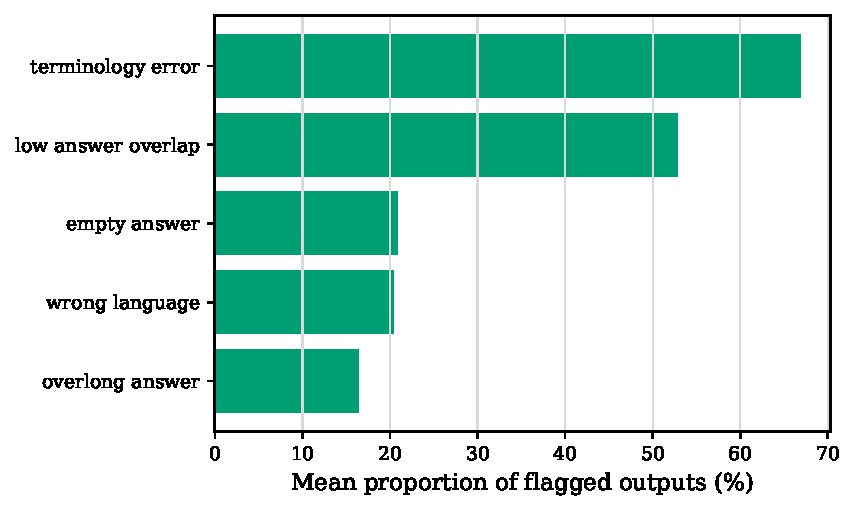
\includegraphics[width=0.96\linewidth,height=\textheight,keepaspectratio]{../paper/ijwis/figures/error_type_distribution.pdf}
\caption{Mean prevalence of automatically flagged output errors.}
\end{figure}

\section{Discussion}\label{discussion}

\subsection{Answers to the research
questions}\label{answers-to-the-research-questions}

\textbf{RQ1 concerned bilingual retrieval.} Lexical and semantic
retrieval are language-dependent complements. Dense retrieval
contributes most to Chinese recall, while exact terminology makes BM25
particularly competitive in English. Approved hybrid fusion reaches the
highest Recall@5 in both languages, but its approximately threefold
latency relative to BM25 means lexical retrieval remains a credible
low-cost configuration. This result is consistent with the broader
rationale for combining retrieval signals rather than assuming semantic
embeddings dominate exact technical language (Robertson and Zaragoza,
2009; Cormack et al., 2009).

\textbf{RQ2 concerned retrieval strategy, governance and answer
behaviour.} RAG improves answer overlap for every generator, but
stronger retrieval recall does not always yield the highest F1. QLoRA
and RAG are complementary for answer content but not automatically for
traceability: adaptation reduces the marginal F1 gain from retrieval and
can overwrite citation-format behaviour. This qualifies railway domain
systems that report aggregate accuracy gains from fine-tuning or RAG (Li
et al., 2024; Luo et al., 2025; Huang et al., 2026). Citation-aware
targets, constrained citation insertion or post-generation entailment
checking are required before operational use.

The approved-only and unfiltered hybrid conditions are identical because
every admissible record in the frozen production index was already
approved. This confirms enforcement of the governance boundary but does
not estimate the causal quality benefit of review. Such an estimate
would require a deliberately retained, ethically usable unreviewed
comparison corpus. The contribution here is therefore the executable
review-state mechanism and its auditability, not a causal claim that
approval alone raises F1.

\textbf{RQ3 concerned bilingual adaptation and translation.}
Completion-only QLoRA substantially improves held-out QA, particularly
for Qwen, but adaptation quality is task-specific. QA gains coexist with
asymmetric Qwen translation regressions and severe GLM
sentence-translation failure. This mirrors concerns that domain-limited
fine-tuning can overfit task form or translation direction (Hu et al.,
2024; Vieira et al., 2024). The practical implication is that QA,
terminology translation, sentence translation and citation compliance
need independent acceptance thresholds; no pooled bilingual score can
justify deployment.

\textbf{RQ4 concerned constrained deployment.} Every tested condition
fits a 24 GB workstation, confirming that a governed local service does
not require a data-centre accelerator. Nevertheless, an adapter's small
file size does not imply lower runtime memory: both QLoRA variants
reserve substantially more memory and generate more slowly than their
quantised base models. Resource reporting must therefore include
measured inference behaviour, not only trainable parameter counts. This
finding complements PEFT literature that emphasises training efficiency
while showing that deployed cost remains model- and backend-dependent
(Ding et al., 2023; Lv et al., 2024).

\subsection{Implications for Web information-system
design}\label{implications-for-web-information-system-design}

The principal theoretical implication is that domain knowledge
enhancement should be evaluated as an information-system pipeline rather
than a single-model treatment. Record governance determines admissible
evidence; retrieval determines whether that evidence is present;
generation determines whether it is used; and the interface determines
whether provenance is visible. Reporting only final answer overlap
collapses these distinct failure modes. The layered protocol used here
reveals, for example, that hybrid retrieval can improve recall without
maximising answer F1, and that adaptation can improve F1 while nearly
eliminating citation-format compliance.

The architecture also treats relational and vector data as
complementary. PostgreSQL remains the authoritative store for source
identity, review state and test exclusion, while pgvector adds semantic
access without replacing those controls. This arrangement is suitable
for institutional Web information systems whose regulations, teaching
materials and language fields evolve over time. It permits a record to
be revised or withdrawn through ordinary data governance while
preserving reproducible model and embedding versions.

\section{Practical implications}\label{practical-implications}

The architecture can support institutions that need local control of
teaching resources and cannot rely on an external hosted model.
PostgreSQL review status, source metadata and held-out flags make
governance rules executable at retrieval time. On a 24 GB workstation,
original Qwen is the practical low-cost option, Qwen QLoRA is preferred
when answer overlap is the priority, and a citation-compliant original
model should remain in the workflow when source display is mandatory.
Teachers should inspect evidence and citations rather than treating
either F1 or citation presence as correctness. International-student
interfaces should retain both source language and translated fields
because retrieval and translation errors are direction-specific.

Deployment can be staged without retraining the entire system. In the
first stage, institutions can expose reviewed BM25 retrieval and
bilingual source display, which offers the lowest latency and preserves
direct evidence access. In the second stage, BGE-M3 and hybrid fusion
can be enabled for questions whose wording differs from source
terminology. In the third stage, local generation can be added with
explicit no-evidence behaviour and teacher-visible citations. Adapted
models should enter service only after passing separate QA, citation and
translation gates. This staged path reduces the risk of treating
generative output as the system of record.

Role-specific interfaces are also important. International learners need
language selection, concise answers and side-by-side source evidence.
Teachers need record editing, source-page inspection, review status and
revision history. Administrators need index coverage, model revision,
latency, memory and failed-generation monitoring. Because the underlying
record identifier is preserved across these views, feedback can be
attached to the responsible knowledge item rather than disappearing into
an untraceable chat log.

For railway education, the system should be framed as decision and
learning support rather than an authority for live safety-critical
action. A visible source citation allows a teacher or learner to consult
the controlling regulation, but neither a citation label nor an
automatic F1 score establishes current legal or operational validity.
Version dates, withdrawal state and responsible reviewer should
therefore remain visible when the knowledge base is updated.

\section{Limitations}\label{limitations}

The held-out set covers four source documents and 17 task types, but it
remains specific to one railway vocational knowledge base and cannot
represent every course, regulation version or learner need. The database
approval field is an operational governance control; the present
experiment does not establish inter-rater agreement or claim that every
approved answer reaches expert consensus. Expert panel composition and
review-protocol metadata are intentionally pending collection and must
be completed before submission. Because the frozen index contains only
approved admissible records, the experiment cannot quantify an
approved-versus-unreviewed quality effect. Automatic F1 penalises valid
paraphrases, while citation presence and the hallucination proxy do not
establish that a citation entails the generated claim. The error
analysis is rule-based and no new human scoring was conducted.
General-benchmark checks were capped per subtask. The experiment uses
one workstation and results should not be generalised to production
concurrency without load testing.

The study also does not measure learner outcomes, usability,
concurrent-user throughput or long-term knowledge-maintenance cost. The
five generators do not represent all current multilingual models, and
the one-epoch rank-64 setting does not establish an optimal PEFT
configuration. Some source passages cannot be redistributed because of
third-party rights, limiting full public replication of the corpus even
though split hashes, scripts and aggregate results can be released.
Finally, cross-backend speed comparisons between Hugging Face and Ollama
are descriptive rather than controlled systems benchmarks.

\section{Conclusion}\label{conclusion}

This study demonstrates a bilingual railway education Web information
system that combines governed PostgreSQL records, pgvector/BGE-M3
retrieval and local generation. Hybrid retrieval achieved the strongest
final recall in both languages, while Qwen2.5 QLoRA produced the
strongest held-out QA and RAG answer-overlap scores within a 24 GB GPU
limit. The same adaptation weakened citation compliance and did not
consistently improve translation; GLM QLoRA failed substantially on
sentence translation. The principal design implication is therefore not
to choose between adaptation and RAG, but to govern them as separate,
testable components with language-, task- and traceability-specific
acceptance criteria.

The contribution to Web information systems lies in making those
acceptance boundaries executable: reviewed records, held-out exclusions,
embedding revisions and evidence provenance are represented in the data
and retrieval layers rather than left to a language-model prompt. Future
work should complete the documented expert-panel metadata, add
citation-entailment and learner-centred evaluation, and test concurrent
service operation across additional railway curricula and language
pairs.

\section{Declarations}\label{declarations}

\textbf{Data availability:} Evaluation scripts, experiment
configurations, aggregate metrics and non-copyrighted derived test
identifiers will be made available with the article. Full source
passages from textbooks and regulations cannot be redistributed where
third-party copyright or licensing restrictions apply; access to those
materials is subject to the original rights holders.

\textbf{Ethics and consent:} No learner personal data are used in the
current experiments.

\textbf{Conflict of interest:} The authors declare no conflict of
interest.

\textbf{Funding:} {[}To be completed before submission: funding body,
grant number and funder's role; state ``This research received no
external funding'' only after confirmation by all authors.{]}

\textbf{Author contributions:} {[}To be completed before submission
using the CRediT taxonomy after the final author list and contribution
allocation are confirmed.{]}

\textbf{Acknowledgements:} Omitted from the anonymous manuscript. Any
non-author expert or institutional acknowledgement will be supplied as a
separate title-page file after contributor consent is confirmed.

\textbf{Use of generative AI:} Generative AI tools were used to assist
code development, result organisation and language editing. The authors
designed the study, executed the experiments, checked the source data
and numerical results, and take responsibility for the final manuscript.
This statement will be reconciled with Emerald's policy in force at the
time of submission.

\section{References}\label{references}

Barnett, S., Brannelly, Z., Kurniawan, S. and Wong, S. (2024),
``Fine-tuning or fine-failing? Debunking performance myths in large
language models'', arXiv:2406.11201, doi: 10.48550/arXiv.2406.11201.

Chen, J., Xiao, S., Zhang, P., Luo, K., Lian, D. and Liu, Z. (2024),
``BGE M3-Embedding: Multi-lingual, multi-functionality,
multi-granularity text embeddings through self-knowledge distillation'',
arXiv:2402.03216.

Chang, Y., Wang, X., Wang, J., Wu, Y., Yang, L., Zhu, K., Chen, H., Yi,
X., Wang, C., Wang, Y., Ye, W., Zhang, Y., Chang, Y., Yu, P.S., Yang, Q.
and Xie, X. (2024), ``A survey on evaluation of large language models'',
\emph{ACM Transactions on Intelligent Systems and Technology}, Vol. 15
No.~3, pp.~1-45, doi: 10.1145/3641289.

Cormack, G.V., Clarke, C.L.A. and Buettcher, S. (2009), ``Reciprocal
rank fusion outperforms Condorcet and individual rank learning
methods'', \emph{Proceedings of the 32nd International ACM SIGIR
Conference}, pp.~758-759.

Dettmers, T., Pagnoni, A., Holtzman, A. and Zettlemoyer, L. (2023),
``QLoRA: Efficient finetuning of quantized LLMs'', \emph{Advances in
Neural Information Processing Systems}, Vol. 36.

Ding, N., Qin, Y., Yang, G., Wei, F., Yang, Z., Su, Y., Hu, S., Chen,
Y., Chan, C.-M. and Chen, W. (2023), ``Parameter-efficient fine-tuning
of large-scale pre-trained language models'', \emph{Nature Machine
Intelligence}, Vol. 5 No.~3, pp.~220-235, doi:
10.1038/s42256-023-00626-4.

Hu, T., Zhang, P., Yang, B., Xie, J., Wong, D.F. and Wang, R. (2024),
``Large language model for multi-domain translation: benchmarking and
domain CoT fine-tuning'', \emph{Findings of the Association for
Computational Linguistics: EMNLP 2024}, pp.~5726-5746, doi:
10.18653/v1/2024.findings-emnlp.328.

Huang, L., Liu, Z., Yu, C., Zhu, T. and Yan, B. (2026), ``Emergency
operation scheme generation for urban rail transit train door systems
using retrieval-augmented large language models'', \emph{Sensors}, Vol.
26 No.~6, 2006, doi: 10.3390/s26062006.

Kasneci, E., Sessler, K., Küchemann, S., Bannert, M., Dementieva, D.,
Fischer, F., Gasser, U., Groh, G., Günnemann, S., Hüllermeier, E.,
Krusche, S., Kutyniok, G., Michaeli, T., Nerdel, C., Pfeffer, J.,
Poquet, O., Sailer, M., Schmidt, A., Seidel, T., Stadler, M., Weller,
J., Kuhn, J. and Kasneci, G. (2023), ``ChatGPT for good? On
opportunities and challenges of large language models for education'',
\emph{Learning and Individual Differences}, Vol. 103, 102274.

Lahnalampi, A. (2024), \emph{Utilizing Large Language Models in Rail
Design Projects}, Master's thesis, Aalto University, available at:
https://aaltodoc.aalto.fi/items/87b7ac34-756c-4db2-8bea-f9b9e6b453ed.

Li, J., Li, C., Niu, S. and Dai, B. (2024), ``RSChat: intelligent
question answering model for railway safety knowledge'', \emph{2024
IEEE/ACIS 24th International Conference on Computer and Information
Science}, pp.~55-60, doi: 10.1109/ICIS61260.2024.10778327.

Lewis, P., Perez, E., Piktus, A., Petroni, F., Karpukhin, V., Goyal, N.,
Küttler, H., Lewis, M., Yih, W.-t., Rocktäschel, T., Riedel, S. and
Kiela, D. (2020), ``Retrieval-augmented generation for
knowledge-intensive NLP tasks'', \emph{Advances in Neural Information
Processing Systems}, Vol. 33, pp.~9459-9474.

Luo, Y.C., Xun, J., Wang, W., Zhang, R.Z. and Zhao, Z.C. (2025), ``A
driver advisory system based on large language model for high-speed
train'', arXiv:2501.07837, doi: 10.48550/arXiv.2501.07837.

Lv, K., Yang, Y., Liu, T., Guo, Q. and Qiu, X. (2024), ``Full parameter
fine-tuning for large language models with limited resources'',
\emph{Proceedings of the 62nd Annual Meeting of the Association for
Computational Linguistics}, pp.~8187-8198, doi:
10.18653/v1/2024.acl-long.445.

Robertson, S. and Zaragoza, H. (2009), ``The probabilistic relevance
framework: BM25 and beyond'', \emph{Foundations and Trends in
Information Retrieval}, Vol. 3 No.~4, pp.~333-389.

Song, Y., Tang, Y. and Liu, R. (2025), ``Large language model and
application for railway track management based on domain
specialization'', \emph{The Proceedings of the 11th International
Conference on Traffic and Transportation Studies}, Vol. 616,
pp.~194-204, doi: 10.1007/978-981-97-9644-1\_21.

Tian, K., Mitchell, E., Yao, H., Manning, C. and Finn, C. (2024),
``Fine-tuning language models for factuality'', \emph{International
Conference on Learning Representations}.

UNESCO (2023), \emph{Guidance for Generative AI in Education and
Research}, UNESCO, Paris.

Vieira, I., Allred, W., Lankford, S., Castilho, S. and Way, A. (2024),
``How much data is enough data? Fine-tuning large language models for
in-house translation'', \emph{Proceedings of the 16th Conference of the
Association for Machine Translation in the Americas}, pp.~236-249.

Wandelt, S., Zheng, C., Wang, S., Liu, Y. and Sun, X. (2024), ``Large
language models for intelligent transportation: a review of the state of
the art and challenges'', \emph{Applied Sciences}, Vol. 14 No.~17, 7455,
doi: 10.3390/app14177455.

Wang, H. and Li, Y.-F. (2024), ``Large-scale language models for PHM in
railway systems: potential applications, limitations, and solutions'',
\emph{Proceedings of the 6th International Conference on Electrical
Engineering and Information Technologies for Rail Transportation}, Vol.
1137, pp.~591-599, doi: 10.1007/978-981-99-9311-6\_59.

Wang, L., Chen, S., Jiang, L., Pan, S., Cai, R., Yang, S. and Yang, F.
(2025), ``Parameter-efficient fine-tuning in large language models: a
survey of methodologies'', \emph{Artificial Intelligence Review}, Vol.
58 No.~8, 227, doi: 10.1007/s10462-025-11236-4.

Zheng, J., Hong, H., Liu, F., Wang, X., Su, J., Liang, Y. and Wu, S.
(2024), ``Fine-tuning large language models for domain-specific machine
translation'', arXiv:2402.15061, doi: 10.48550/arXiv.2402.15061.

Zheng, O., Abdel-Aty, M., Wang, D., Wang, C. and Ding, S. (2023),
``TrafficSafetyGPT: tuning a pre-trained large language model to a
domain-specific expert in transportation safety'', arXiv:2307.15311,
doi: 10.48550/arXiv.2307.15311.
